\documentclass[
	%a4paper, % Use A4 paper size
	letterpaper, % Use US letter paper size
]{jdf}

\addbibresource{references.bib}

\author{Chris Messer}
\email{cmesser31@gatech.edu}
\title{Pandemic Simulation}

\begin{document}
%\lsstyle

\maketitle

\begin{abstract}
Seasonal influenza outbreaks pose significant health and economic burdens annually. This paper employs a simulation-first approach to investigate influenza transmission dynamics and assessing mitigation strategies.  Herein, we introduce a computational model and analyze simulation outcomes of a flu virus in a small classroom environment . We also explore the effectiveness of intervention measures such as vaccination, to inform evidence-based strategies for seasonal outbreak control. Through the methods outlined in this report, we conclude a 50\% vaccination rate was found to be an effective method of reducing the number of days the flu virus was present in the environment by a mean of 3.48 days. 
\end{abstract}

\section{INTRODUCTION}
According to the Centers for Disease Control and Prevention, the Flu is a contagious respiratory illness caused by influenza viruses that infect the nose, throat, and sometimes the lungs \citep{cdc}. Understanding the mechanisms of influenza transmission in such settings is crucial for implementing effective prevention and control measures, and swaying public perception of the effectiveness of these measures.

This paper approaches the analysis of infectious disease propagation through a simulation-first approach, and subsequently analyzes the simulation results with statistical rigour. The remainder of this paper is organized as follows: Section 2) Simulation methods and assumptions, and the mathematical underpinning of the computational model; Section 3) Analysis of the simulation through examination of several key metrics; Section 4) Simulation exploration of various disease propagation reductions methods such as vaccination prevalence. 

Central to our methodology is the development of a simple yet versatile model for simulating flu pandemics. This model is underpinned by a set of assumptions that can be readily adjusted to accommodate different scenarios and evaluate the robustness of our findings under varying circumstances. Through a synthesis of simulation-based experimentation and rigorous statistical analysis, we aspire to contribute meaningfully to the collective effort aimed at safeguarding public health in the face of infectious disease threats.
\section{METHODS}
The construction of the simulation model followed a process-interaction framework, aiming to capture the dynamic interactions between students within a classroom setting. The model was implemented using Python programming language, leveraging its versatility and extensive libraries for scientific computing and visualization.

\subsection{Assumptions}
In our classroom model, several assumptions were made. Specifically, the simulation sought to describe a classroom of 31 elementary school kids, with 30 healthy students, and 1 infected student, aliased as \textit{Tommy} for the remainder of this report. Tommy enters the classroom on day 1 (\(D_1\)) while infected with a flu virus that has a 2\% chance of transmission (\(P_{t} = .02\)). Once infected on Day \(D_i\), the student is contagious for the following three days, \(D_{i+1} ... D_{i+3}\). It is assumed that every student is present every day at school, regardless of whether they are infected, contagious or healthy. The simulation trial runs until there are no more contagious students.

For the base case of the simulation as discussed in the \textit{Analysis} section, it is assumed that no precautionary measures such as vaccinations are taken.

\subsection{Process Interaction}
As described in the \textit{Introduction} section, the simulation model uses a process-interaction approach to modeling. That it, within the simulation code, classroom and student entities are defined and initialized with parameters to model our desired simulation system.

\subsubsection{Students}
At the beginning of each simulation trial, students are initialized with the below parameters:
\begin{itemize}
\item \textit{Probability of transmission (\(P_{t}\)) -} this is a value between 0 and 1. A value of 0\% implies the student is not contagious, and has a 0\% chance of infecting other students. A value of 1 would imply a the student is very contagious and will infect 100\% of students they come in contact with. For purposes of this simulation, it is assumed that every student in the classroom is in contact with every other student, every day of the simulation. This value is initialized as .02.
\item \textit{Probability of being vaccinated (\(P_v\)) -} this is a value between 0 and 1. A uniform random variable \(U\) is generated using the numpy python package \citep{harris2020array}. If \(U <P_v\), then the student is considered vaccinated and a parameter \(V\) is initialized as 1, or 0 if the student is not vaccinated. This is initialized as 0 for the base case analysis.
\item  \textit{Vaccine effectiveness (\(P_{ve}\)) -} this is an initialized value between 0 and 1 that represents the effectiveness of the vaccine, if the student is vaccinated. A value .5 corresponds to an 50\% reduction in chance that a student is infected when exposed. In the context of this simulation, if a student is exposed to a virus with \(P_{t} = .02\), and \(P_{ve} = .5\), then the student has a \(.02*.5 = .01\) or \(1\%\) of being infected.
\end{itemize}
\subsubsection{Classroom}
At the start of each simulation trial,  a classroom is also initialized with the following parameters:

\begin{itemize}
    \item \textit{Students -} This represents a list of students who are present in the classroom. Each student in the list is individually initialized with their own values of the parameters defined above. 
\end{itemize}

First, the probability that a single non-infected student will become infected is determined as \(P_t\). Then, we determine the probability that any non-infected student is \textit{not} infected (expressed as \(\phi\)) by any of the other \(I_i\) number of infected students, calculated as:
\[\phi =({1-P_t})^{I_i}\]
where \(I_i\) is the total number of infected students on day \(i\). The value  \(1-\phi_i = \Phi_i\) now represents the probability that any non-infected student will become infected on \(i^{th}\) day of class. Then, we calculate the probability \(\beta\) that an individual student is going to become infected by considering the overall risk of being infected (\(\Phi_i\)) on day \textit{i} reduced by the students vaccination status and the pre-determined vaccine effectiveness:
\[\beta = \Phi_i(1-P_{ve}V)\]
Finally, a trial is then performed for each student considering their probability of getting infected \(\beta\), which considers their individual vaccination status, the vaccine effectiveness, and the overall classroom exposure risk \(\beta\). A random variable \textit{U} is generated using numpy and compared to \(\beta\), and if \(U \leq \beta\), the student is considered infected on \(D_i\) and will be contagious for days \(D_{i+1}... D_{i+3}\). \citep{harris2020array}


\section{ANALYSIS}
Following the methods described above, the simulation model was run, with \(P_{t} = .02,P_{v}=0, P_{ve}=0\), with Tommy as the only infected student on \(D_1\). In other words, the a contagious student had a 2\% chance of infecting non-infected students, and no students were vaccinated. The model was run for ten thousand trials.

To analyze the results of the model, several metrics were calculated as described below. Each metric is observed through the resulting dataset from the model, and then determined analytically for comparison. 

\subsection{Distribution of students infected on \(D_1\)}
\subsubsection{Observed}
Our first step in analyzing the distribution of students who became infected on \(D_1\) is creating a subset of the data generated by the simulation output. The accompanying notebook contains the code used to pivot and summarize the model output under the base case assumptions, and was then plotted as a histogram. 

\begin{jdffigure}
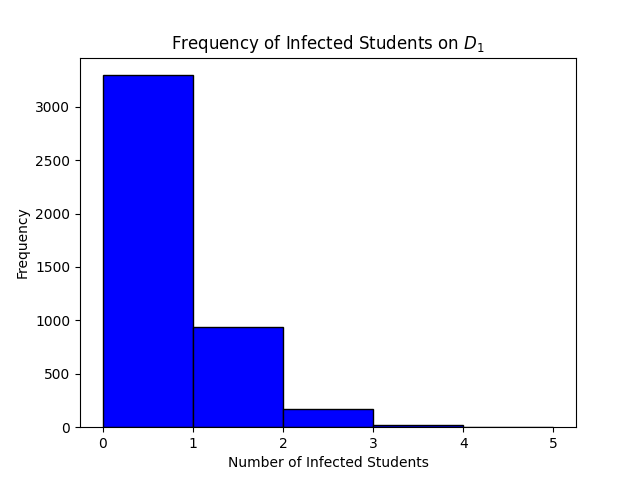
\includegraphics[height=6cm]{Figures/q1_hist.png}%
\captionof{figure}{The observed frequency of students infected on \(D_1\) appears to follow a binomial distribution}
\end{jdffigure}

Before examining our data analytically to determine the distribution, we consider the nature of our data. Ultimately, a student getting infected with probability \(P_t\) can be considered a Bernoulli trial. Then, consider the simulation on one day measuring how many successes there are of individual Bernoulli trials, which by definition, is a Binomial Distribution. \citep{goldsman2020}

The Binomial Distribution has two parameters, number of trials \textit{n}, and probability of success \textit{p}. In our case, we know the probability of success is the probability that a student is infected, which we have denoted as \(P_{t}\) in the base case assuming no vaccinations. Further, the number of \textit{n} trials is equal to the number of students susceptible to infection on \(D_1\), which in this case, is 30. 

Thus, we hypothesize that the number of students infected on \(D_1\) follows a Binomial(\(n = 30, p = .02\)) distribution. 
\subsubsection{Expected}
To test our hypothesis, we first generate random data that follows a Binomial(\(n = 30, p = .02\)) distribution. To do this, we consider the binomial probability distribution function \citep{goldsman2020}:
\[f(x) = \left(\begin{array}{l}
n \\
x
\end{array}\right) p^x(1-p)^{n-x}\]
where \(x\) is the count of infected students, \textit{n} is the number of susceptible students, and \textit{p} is the probability of infecting other students, or \(P_t\). In the accompanying notebook, we calculate the expected percent of observations that we would expect to see \(x\) of infected students, and multiplied this by the number of simulation trials to get comparable number of simulations. 

These values represent the percent of observations expected to fall into each value of \(x\), or what percent of trials we should expect to see \(x\) number of student become infected on day \(D_1\). We then multiply these percentages by the number of trials we simulated, to get a numerical approximation. Lastly, we plot these expected values against our observed values in figure 2 below.

\begin{jdffigure}
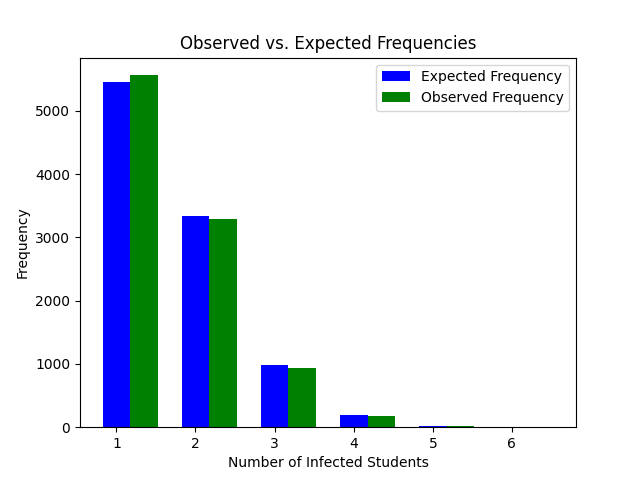
\includegraphics[height=6cm]{Figures/q2_hist_obs_vs_exp.png}%
\captionof{figure}{The observed frequency closely matches the expected frequency}
\end{jdffigure}

Our observed values of \textit{x} appear to follow the expected Binomial(\(n = 30, p = .02\)) distribution, but we can formally test our hypothesis by using a \(\chi^2\) goodness of fit test. Our null hypothesis \(H_0\) is that the observed number of students infected on \(D_1\) follows a Binomial(\(n = 30, p = .02\)) distribution. To perform this test, we first calculate our \(\chi^2\) value as \citep{goldsman2020}:
\[\chi^2=\sum \frac{\left(O_i-E_i\right)^2}{E_i}\]
where \(O_i\) is the \(i^{th}\) observed value and \(E_i\) is the \(i^{th}\) expected value. In the accompanying code workbook, it is found that the \(\chi^2\) test statistic is 7.01.


Then, the significant value of \(\chi_\alpha^2\) is found by referencing a \(\chi^2\) chart. For a \(\alpha = .05\) level of significance with \(n-1 =5\) degrees of freedom, the significant value of \(\chi_\alpha^2= .05\) is 11.07 \citep{goldsman2020}. As \(\chi^2 < \chi_\alpha^2\), we conclude there is not enough evidence to reject the null hypothesis, and we conclude that the distribution of students infected on day 1 follows a Binomial(\(n = 30, p = .02\)) distribution. 

\subsection{Expected number of students infected on \(D_1\)}
\subsubsection{Observed}
The expected number of students Tommy infects on day one can be estimated using the simulation, by simply taking the average number of students infected on \(D_2\) (where \(D_1\) is the first day that Tommy came to school) across all trials. Note, this value includes Tommy himself as he is also infected on Day 2.

 We note the sample mean is an unbiased estimator for the population mean. \citep{goldsman2020} Through observing our simulation output, we conclude that over the ten-thousand simulated classroom trials, on \(D_1\) there was an average of 1.58 students infected. 

\subsubsection{Expected}
The expected value of students infected on \(D_1\) (notated as \(\overline{I}_1\)) can be calculated analytically as well. The expected value of a binomial distribution is determined by \[\overline{I}_1 = E[X]=np\] where n is the number of students susceptible to infection on \(D_1\) (\(n=30\)), and \(p\) is the probability of transmission, or \(P_{t}=.02\). As such, we conclude the expected number of students infected on \(D_1\) to be 1.6, close to our observed value. \citep{goldsman2020}

\subsection{Expected number of students infected on \(D_2\)}
\subsubsection{Observed}
Similar to the above, we can observe the expected number of students infected on \(D_2\) by observing the mean number of students infected on \(D_2\) in our simulation output. On \(D_2\), we observe there are 2.46 students infected on average on \(D_2\)

\subsubsection{Expected}
The expected number of students infected on \(D_2\) can also be derived analytically, however, this will require additional calculations and considerations, as the number of infected students on \(D_2\) is dependent on the number of infected students on \(D_1\). This problem can be decomposed into several sub-problems. By the law of the unconscious statistician, the expected value of students infected on \(D_2\) can be formalized as 
\[\overline{I}_2 = E[X_2]= \sum_{i=1}^{n}x_2f(x_i)\]
where \(x_2\) is the number of students infected on \(D_2\), \(n\) is the number of susceptible students to infection on \(D_2\), \(\overline{I_i}\) is the expected number of students infected on \(D_i\), and \(f(x)\) is the probability there are \(x\) number of students infected on \(D_2\). 

\(f(x)\) is dependent on \(\overline{I}_1\), since more students infected on \(D_1\) would increase the probability of infection on \(D_2\). This relationship is formalized as
\[f(x) = \left\{\begin{matrix}
P(I_2 = 0\cap I_1=0) & x=0\\ 
P(I_2 = 1\cap I_1=0)+P(I_2 = 0\cap I_1=1) & x=1\\ 
P(I_2 = 0\cap I_1=2)+P(I_2 = 1\cap I_1=1)+P(I_2 = 2\cap I_1=0) & x=2\\ 
...

\end{matrix}\right.\]
for all values of \(x \in \{0,1,... n\}\) where \(n\) is the number of  students susceptible to infection, and \(f(x)\) defines the probability there are \(x\) infected students on \(D_2\). \(f(x)\) can be generalized, as this ultimately represents the cumulative probability for all the possible ways there can be \(x\) students infected on \(D_2\). For example, if \(x=2\) on \(D_2\), this could be a result of:
\begin{itemize}[noitemsep]
    \item 0 students infected on \(D_1\) and 2 students infected on \(D_2\)
    \item   1 students infected on \(D_1\) and 1 students infected on \(D_2\)
    \item 2 students infected on \(D_1\) and 0 students infected on \(D_2\)
\end{itemize}


As such, \(f(x)\) is generalized as:
\[f(x) = \sum_{n=0}^{x}P\left (I_2 = (x-n)\cap I_1=n  \right )\]

The intersecting probability \(P(I_2 = i_2\cap I_1=i_1)\) can be determined by the conditional probability formula: \[P(A\cap B) = P(A|B)P(B)\]
\(P(B)\) is representing the probability of \(i_1\) students being infected on \(D_1\) (\(I_1 = i_1\)). We have previously concluded our infection probability follows a binomial distribution, so we can calculate this using the probability density formula for a Binomial(\(n = 30, p = .02\)) distribution:
\[P(B) = P(I_1 = i_1) = \left(\begin{array}{l}
n_1 \\
i_1
\end{array}\right) p^{i_1}(1-p)^{n_1-i_1}\]
where \(n_1\) is the number of susceptible students on \(D_1\), and \(p\) is the probability of transmission, or .02 in the base case, and \(i_1\) is the number of infected students on \(D_1\).

\(P(A|B)\) here is representing the probability of \(A\) (or \(I_2=i_2\)) students getting infected on \(D_2\) given B (or \(I_1=i_1\)) students infected on \(D_1\). This too will follow the binomial distribution, as it is simply a repeating set of Bernoulli trials with different values of \(n\) and  \(i\).
\[P(A|B) = P(I_2 = i_2) = \left(\begin{array}{l}
n_2 \\
i_2
\end{array}\right) p^{i_2}(1-p)^{n_2-i_2}\]
The above set of formulas are formalized into python code in the supplementary notebook to recursively calculate our original objective function \(\overline{I}_2 = E[X_2]= \sum_{i=1}^{n}x_if(x_i)\) for the mean number of students infected on \(D_2\), and was found to be 2.51 students when including Tommy. This closely reflects the observed number of 2.46. 

\subsection{Observed number of students infected on \(D_i\)}
The simulation was run for 30 days, across ten thousand simulations to observe patterns in the length the flu lasted in our simulated classroom, with the intent to have a baseline to compare against different spread reduction methods (vaccines in our case). Under our base case discussed above, the estimated \(\hat{I}\) number of infections on each day \(D_i\) of the simulation were as follows:

\begin{jdffigure}
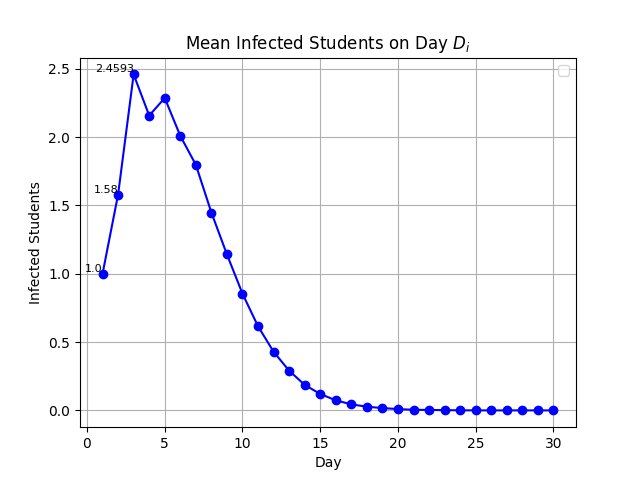
\includegraphics[height=6cm]{Figures/q4a.png}%
\captionof{figure}{The mean infected students on days \(D_i\) match our analysis from above. Subsequent days show a sharp drop off in infected students.}
\end{jdffigure}

This data was then pivoted to show the occurrences of the last day of the flu pandemic across all ten thousand trials, and plotted as a histogram in figure 4 below.

\begin{jdffigure}
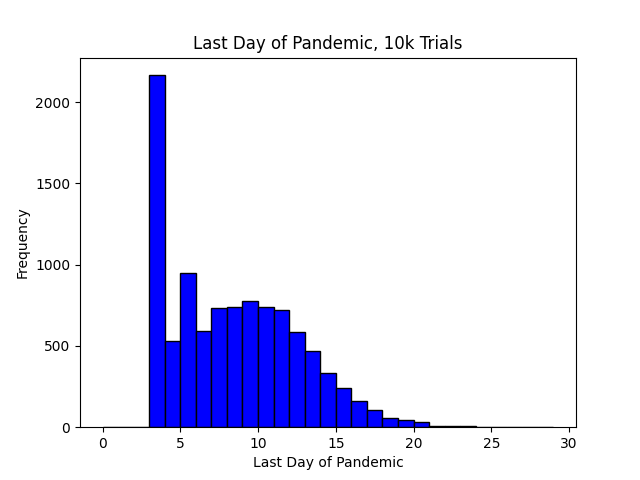
\includegraphics[height=6cm]{Figures/q4b.png}%
\captionof{figure}{The pandemic frequency often has a length of 1, as there is a low probability of any students getting infected the first day. If even one additional student is infected, the pandemic length increases significantly, causing overlapping distributions in the observed pandemic length.}
\end{jdffigure}

\section{Harm Reduction Methods}
In addition to our above analysis, we reran the simulation assuming one out of two students were vaccinated on average, with a 100\% vaccine effectiveness to see the impact on the mean infected students each day and the length of the pandemic. We used the methods described above, and changed only the values of \(P_v\) and \(P_{ve}\) to .5 and 1, respectively. 

With with each student having a 50\% chance of being vaccinated, across ten thousand trial, the mean number of infected students on each day was found to be:

\begin{jdffigure}
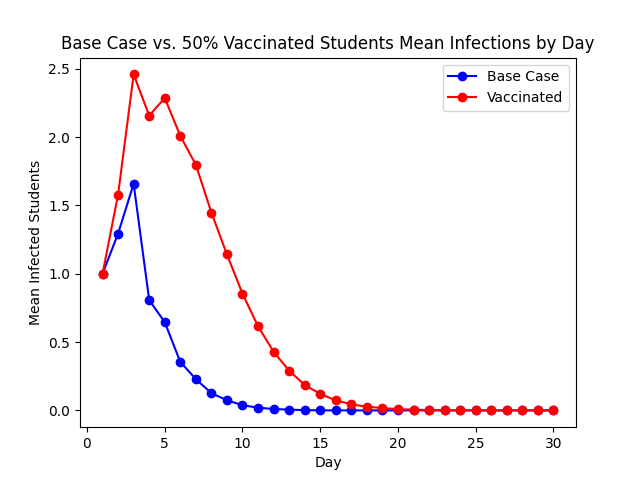
\includegraphics[height=6cm]{Figures/Q5a.png}%
\captionof{figure}{The introduction of vaccines to the student population has a noticeable impact on the mean students impacted each day}
\end{jdffigure}

Then, we examined the length of the pandemic:
\begin{jdffigure}
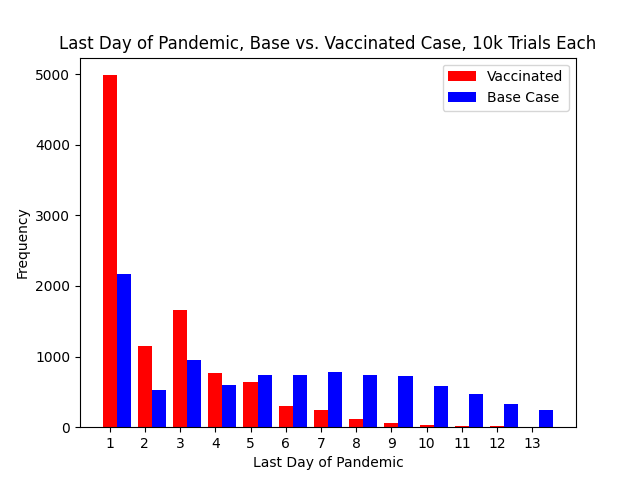
\includegraphics[height=6cm]{Figures/q5c.png}%
\captionof{figure}{A mean 50\% vaccination rate shows significant reduction in the pandemic length}
\end{jdffigure}

\subsection{Mean Comparison}

By observing the simulation outputs from each scenario, we can calculate the mean length of the pandemic for both the vaccinated and base cases. 

These means are independent of one another, and have arbitrary and unknown variances. As such, we can compare them by observing the  approximate confidence interval of the mean difference. First, we calculate the sample variance of each mean:
\[S_Z^2 \equiv \frac{1}{r-1} \sum_{i=1}^r\left(Z_i-\bar{Z}_r\right)^2\]
where Z is either the base or vaccinated scenario (denoted as X and Y here forward, respectively), \(r\) is the number of replications in the simulation (10k in both cases), \(Z_i\) is the length of the pandemic on the \(i^{th}\) replication, and \(\bar{Z}_r\) is the mean pandemic length across all trials. In the accompanying notebook, the sample variances and means are determined as :
\begin{table}
    \centering
    \begin{tabular}{|c|c|l|} \hline 
         Scenario& Mean Pandemic Length (\(\overline{X}, \overline{Y}\))&Sample Variance (\(S_{X}^2,S_{Y}^2\))\\ \hline 
         Base (\(X\))& 7.9 days &16.92\\ \hline 
         Vaccinated (\(Y\))& 4.4 days &3.76\\ \hline
    \end{tabular}
    \caption{Base vs. Vaccinated Mean and Sample Variance of Pandemic Lengths over 10k trials each}
    \label{tab:my_label}
\end{table}

Then, we can compare the means at a 95\% confidence interval through the approximate CI formula \citep{goldsman2020}:
\[\nu \equiv \frac{\left(\frac{S_X^2}{n}+\frac{S_Y^2}{m}\right)^2}{\frac{\left(S_X^2 / n\right)^2}{n+1}+\frac{\left(S_Y^2 / m\right)^2}{m+1}}-2\]
\[\mu_X-\mu_Y \in \bar{X}-\bar{Y} \pm t_{\alpha / 2, \nu} \sqrt{\frac{S_X^2}{n}+\frac{S_Y^2}{m}}\]
Where \(\nu\) is the estimated degrees of freedom, \(n\) and \(m\) are the number of trials of each simulation, and \(t_{\alpha / 2, \nu}\) is the \(t\) critical value for \(\nu\) degrees of freedoms (calculated using the scipy python package \citep{2020SciPy-NMeth}) .
In the accompanying notebook, the difference in means was determined to be 3.48 days, with a 95\% CI within [3.4, 3.55]. 
\section{Conclusion}
This paper presents a simulation-based study on influenza transmission in a classroom setting, focusing on the effectiveness of vaccination. Through Python-based modeling and statistical analysis, we examined transmission dynamics and intervention strategies.
Future research could explore additional factors like varying vaccination effectiveness and compliance rates. Expanding simulations to larger populations or different settings could offer broader insights into public health strategies.

In conclusion, this study highlights the value of simulation modeling and statistical analysis in understanding infectious disease dynamics and guiding preventive measures. Refining our understanding can inform effective public health policies to mitigate influenza outbreaks.

\section{References}
\printbibliography[heading=none]





\end{document}
